\documentclass{article}

\usepackage{graphicx}
\usepackage{tikz}
\usepackage{tikzsymbols}
\usetikzlibrary{calc,patterns,shapes.geometric}
\pagestyle{empty}
\usepackage[margin=0pt]{geometry}
\geometry{papersize={14in,12in}}

\def\centerarc[#1](#2)(#3:#4:#5){\draw[#1] ($(#2)+({#5*cos(#3)},{#5*sin(#3)})$) arc (#3:#4:#5);}

\begin{document}
	\begin{figure}
		\centering
		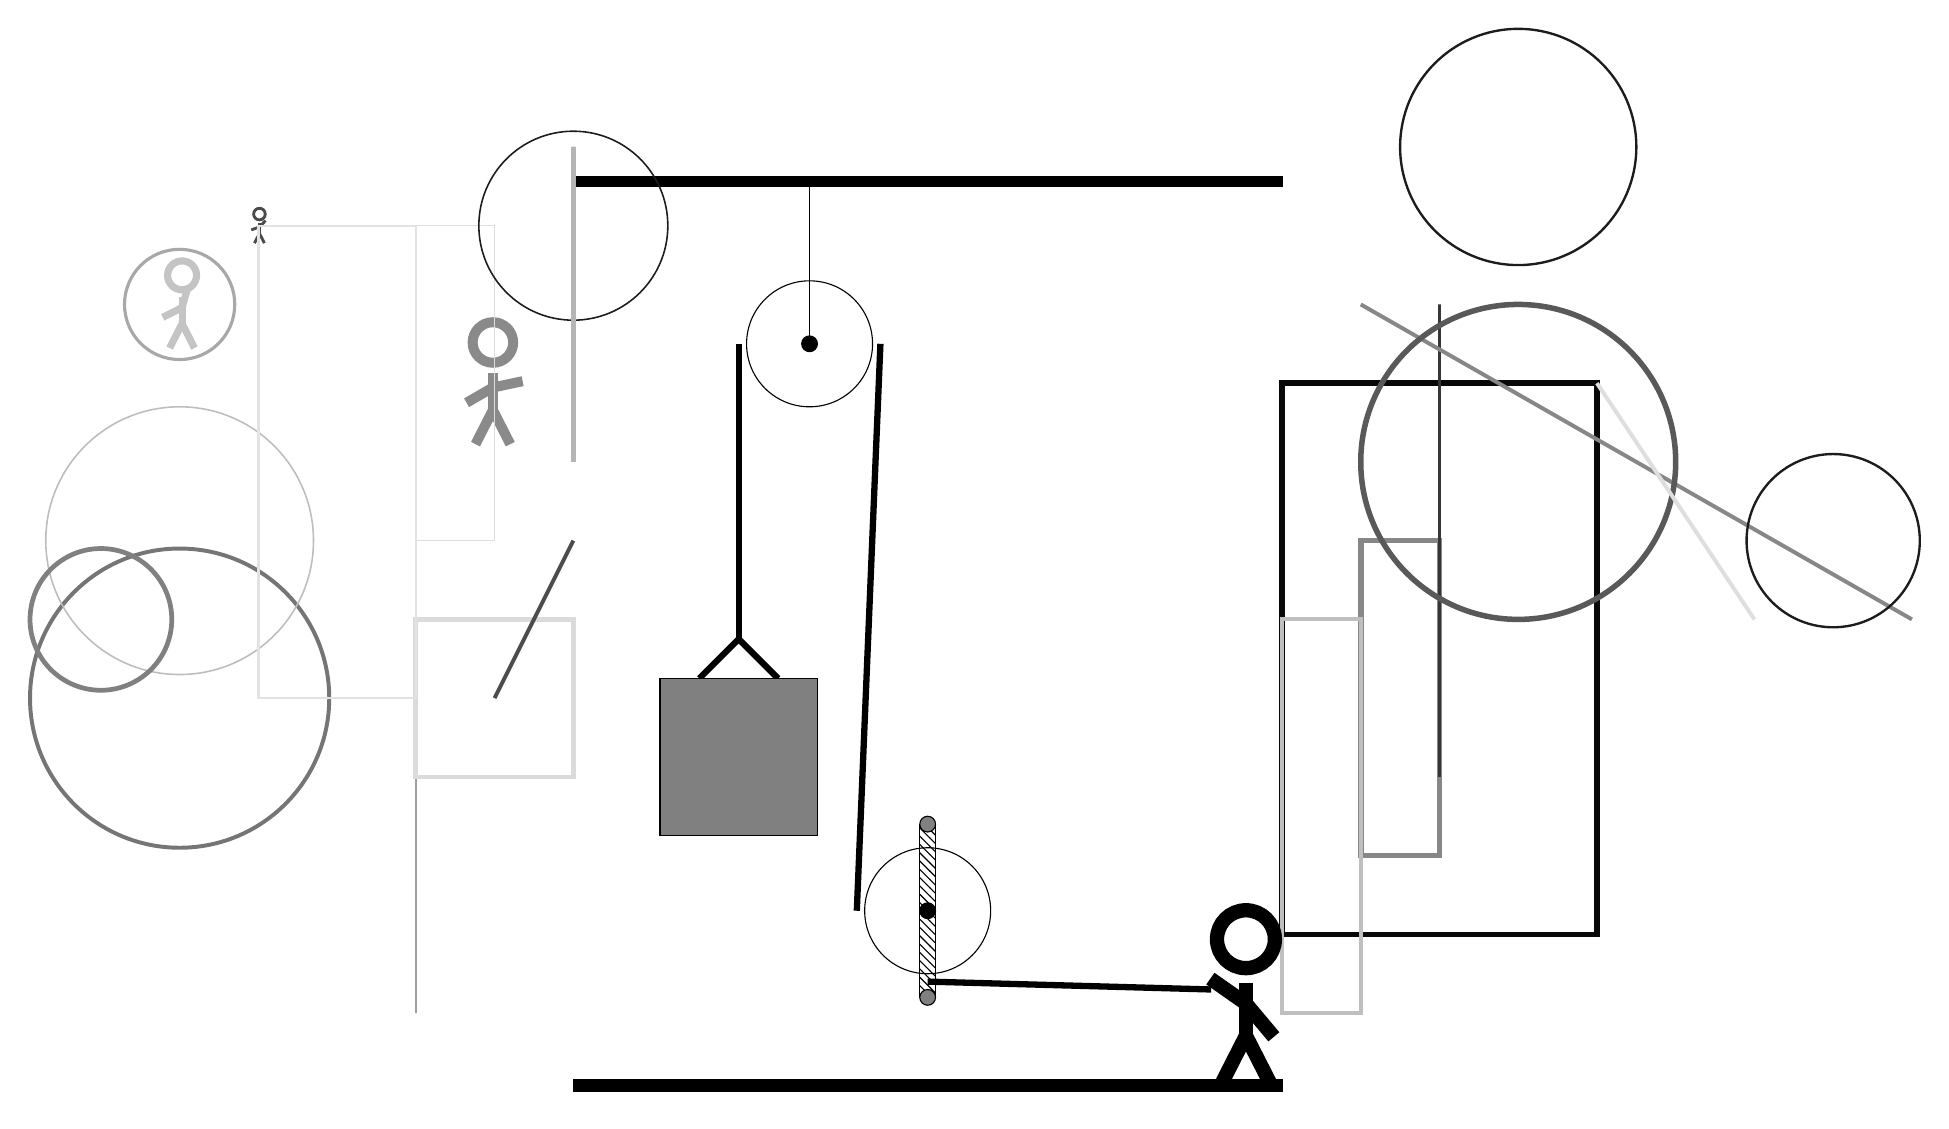
\begin{tikzpicture}
			%%%%% START %%%%%
			
			\draw[fill=black] (-2, 11.5) rectangle (7, 11.625);
			
			\draw (1, 9.5) circle (0.8);
			\draw[fill=black] (1, 9.5) circle (0.1);
			\draw (1, 11.5) -- (1, 9.5);
			
			\node[line width=0.5mm, color=black!46] at (-3, 9) {\Strichmaxerl[7][30][12]};
			
			\draw[line width=0.2mm, color=black!38] (-4, 7) rectangle (-4, 1);
			\draw [line width=0.3mm, color=black!89](10, 12) circle (1.5);
			\draw [line width=0.5mm, color=black!54](-7, 5) circle (1.9);
			\draw[line width=0.7mm, color=black!47] (9, 7) rectangle (8, 3);
			
			\node[line width=0.4mm, color=black!71] at (-6, 11) {\Strichmaxerl[2][20][46]};
			\draw[line width=0.7mm, color=black!97] (7, 2) rectangle (11, 9);
			\draw[line width=0.2mm, color=black!13] (-3, 7) rectangle (-4, 11);
			\draw[line width=0.6mm, color=black!14] (-2, 4) rectangle (-4, 6);
			\draw[line width=0.5mm, color=black!79] (9, 10) rectangle (9, 4);
			\draw[line width=0.5mm, color=black!47](8, 10) -- (15, 6);
			
			\draw [line width=0.7mm, color=black!65](10, 8) circle (2.0);
			\draw[line width=0.5mm, color=black!25] (8, 6) rectangle (7, 1);
			
			\draw[line width=0.5mm, color=black!70](-2, 7) -- (-3, 5);
			\draw[line width=0.4mm, color=black!59] (-2, 12) rectangle (-2, 9);
			\draw [line width=0.2mm, color=black!26](-7, 7) circle (1.7);
			\draw [line width=0.3mm, color=black!89](14, 7) circle (1.1);
			
			\draw [line width=0.2mm, color=black!89](-2, 11) circle (1.2);
			\draw[line width=0.5mm, color=black!13](11, 9) -- (13, 6);
			
			\draw[line width=0.7mm, color=black!29] (-2, 12) rectangle (-2, 8);
			\draw[line width=0.3mm, color=black!11] (-4, 11) rectangle (-6, 5);
			\draw [line width=0.4mm, color=black!34](-7, 10) circle (0.7);
			\draw [line width=0.6mm, color=black!50](-8, 6) circle (0.9);
			\node[line width=0.4mm, color=black!23] at (-7, 10) {\Strichmaxerl[5][27][74]};
			
			\draw[fill=white](2.5, 2.3) circle (0.8);
			\draw[fill=black] (2.5, 2.3) circle (0.1);
			\draw[pattern=north west lines, pattern color=black] (2.4, 3.4) rectangle (2.6, 1.2);
			\draw[fill=black!50] (2.5, 3.4) circle (0.1);
			\draw[fill=black!50] (2.5, 1.2) circle (0.1);
			
			\draw[line width=0.8mm] (-0.4, 5.25) -- (0.1, 5.75) -- (0.6, 5.25);
			\draw[fill=black!50] (-0.9, 5.25) rectangle (1.1, 3.25);
			
			\draw[line width=0.8mm] (0.1, 9.5) -- (0.1, 5.75);
			\centerarc[line width=0.8mm](1, 9.5)(0:180:0.9);
			\draw[line width=0.8mm](1.9, 9.5) -- (1.6, 2.3);
			\centerarc[line width=0.8mm](2.5, 2.3)(180:270:0.9);
			\draw[line width=0.8mm](2.5, 1.4) -- (6.1, 1.3);
			
			\node at (6.5, 1.2) {\Strichmaxerl[10][-35][-50]};
			
			\draw[fill=black] (-2, 0) rectangle (7, 0.15);
			
			%%%%% END %%%%%
		\end{tikzpicture}
	\end{figure}	
\end{document}